\begin{frame}
	\frametitle{SimpIL}
	\vspace{-0.5cm}
	Designed to demonstrate the critical aspects of this analysis. \newline
	\only<1>{
		\begin{center}
			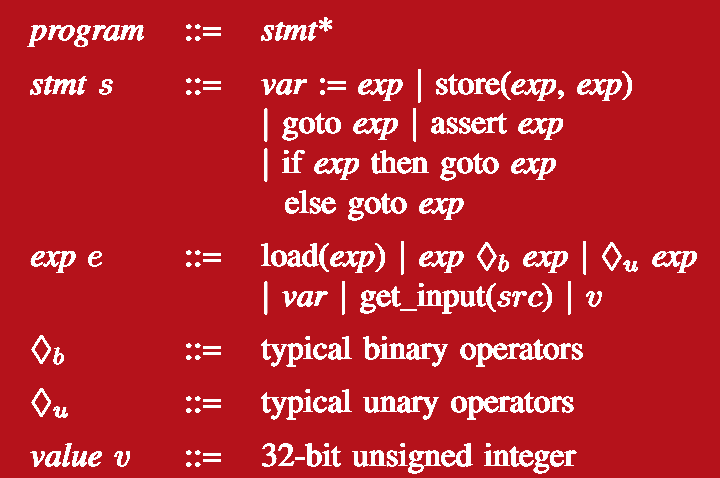
\includegraphics[scale=0.30]{SimpIL}
			\newline
			\textbf{SimpIL Grammar}
		\end{center}
	}
	\only<2>{
		\begin{itemize}
			\item \textbf{Each} statement rule of the operational semantic is like:
		\end{itemize}
		\begin{prooftree}
			\AxiomC{computation}
			\UnaryInfC{$\textless$current state$\textgreater$, stmt $\rightarrow$ $\textless$end state$\textgreater$, stmt’}
		\end{prooftree}
		\begin{itemize}
			\item The \texttt{state} is composed of: \newline
		\begin{minipage}{0.5\textwidth}
			\begin{itemize}
				\item Program statements ($\sum$)
				\item Current memory state ($\mu$)
				\item Current values for variables ($\Delta$)
			\end{itemize}
		\end{minipage}
		\begin{minipage}{0.4\textwidth}
			\begin{itemize}
				\item Program counter (\textit{pc})
				\item Current statement (\textit{i})
			\end{itemize}
		\end{minipage}
	\end{itemize}
	}
\end{frame}